\RequirePackage[T1]{fontenc}
\documentclass[12pt]{article}
\pdfoutput=1 % if your are submitting a pdflatex (i.e. if you have images in pdf, png or jpg format)
\usepackage[height=8.9in,width=6.45in]{geometry}
%\usepackage{showkeys}
\renewcommand{\baselinestretch}{1.06}

\usepackage[utf8]{inputenc}
\usepackage{amsmath}
\usepackage{amssymb}
\usepackage{mathtools}
\numberwithin{equation}{section}
\usepackage{slashed}
\usepackage{braket}
\usepackage[dvipsnames,svgnames,table]{xcolor}
\usepackage[colorlinks,linktocpage=true,citecolor=DarkGreen,linkcolor=FireBrick,urlcolor=FireBrick]{hyperref}
\usepackage{cite}
\usepackage{graphicx}
\usepackage{tikz}
\usepackage{tikz-cd}
\usepackage{times}
\usepackage[scaled]{couriers}
\usepackage{bm}
\usepackage{subfig}
\usepackage{mathrsfs}
\usepackage{amsthm}
\usepackage{sseq}
\usepackage{xypic}
\usepackage{spectralsequences}

\usepackage{mdframed}
\newenvironment{claim}{  \begin{mdframed}[linecolor=black!0,backgroundcolor=black!10]\noindent\itshape\ignorespaces}{\end{mdframed}}

\let\originalfigure=\figure
\let\endoriginalfigure=\endfigure

\renewenvironment{figure}[1][]{
  \begin{originalfigure}[#1]
    \begin{mdframed}[linecolor=black!0,backgroundcolor=black!1]
}{
    \end{mdframed}
  \end{originalfigure}
}

\def\bR{\mathbb{R}}
\def\bZ{\mathbb{Z}}
\def\cP{\mathcal{P}}
\def\Sq{\mathop{\mathrm{Sq}}\nolimits}
\newcommand{\vev}[1]{ \left\langle {#1} \right\rangle }
\def\Nequals#1{$\mathcal{N}{=}#1$}
\def\ind{\mathop{\mathrm{ind}}}
\def\ch{\mathop{\mathrm{ch}}\nolimits}
\def\tr{\mathop{\mathrm{tr}}}
\def\comment#1{\textcolor{red}{#1}}
\def\HP{\mathbb{HP}}

\definecolor{wo}{rgb}{1.0, 0.85, 0.6}
\definecolor{wb}{rgb}{0.7, 0.9, 1.0}
\definecolor{lg}{rgb}{.9,.9,.9}
\def\Sp{Sp}
\def\SU{SU}
\let\BZ\bZ
\def\bC{\mathbb{C}}
%Yuji's macros
%%list witten

\begin{document}

\begin{table}
$M$ is a spin manifold of dimension 4, with $\bC^2\to S\to M$ the spin bundle.
The gauge fields come from the principal bundle \[
SU(3)\times SU(2)\times U(1) \to P\to M,
\] and the matters are the sections of the associated bundle
\[
  \underline{V_\text{boson}} 
  \oplus
  (\underline{V_\text{fermions}}\otimes S)
  \to M,
\]
 \[
V_\text{boson} = \mathbf{2} \otimes V_{+1/2},
\qquad 
  V_\text{fermion}=\bC^3 \otimes V_\text{single generation}
\] where $V_\text{single generation}$ is
\[
\label{eq:generation}
  \begin{array}{ccccccl@{\qquad}lcc}
&  &    \mathbf{3} &\otimes & \mathbf{2} &\otimes& V_{+1/6}  & (\text{the quark doublet} & Q_L) \\
& \oplus&   \mathbf{\bar 3} & & &  \otimes&  V_{-2/3}  & (\text{the up-type antiquark} & \bar u_R) \\
&\oplus &  \mathbf{\bar 3} & & &\otimes& V_{+1/3} & (\text{the down-type antiquark} & \bar d_R) \\
&\oplus  & & & \mathbf{2} &\otimes& V_{-1/2}  & (\text{the lepton doublet} & \ell_L) \\
&\oplus &  & & &\otimes& V_{+1} & (\text{the charged anti-lepton} & \bar e_R)\\
&\oplus &&&&& \bC & (\text{the right-handed neutrino} & \bar \nu_R).
  \end{array}
\]
where $\mathbf{3}$, $\mathbf{2}$ are the standard representations of $SU(3)$ and $SU(2)$,
and $U(1)\curvearrowright V_q\simeq \bC$ is via $z\cdot v = z^{6q} v$ for $z\in U(1)$, $v\in V_q$.
\caption{The bundle content of the Standard Model}
\end{table}

\begin{figure}[h]
\centering   
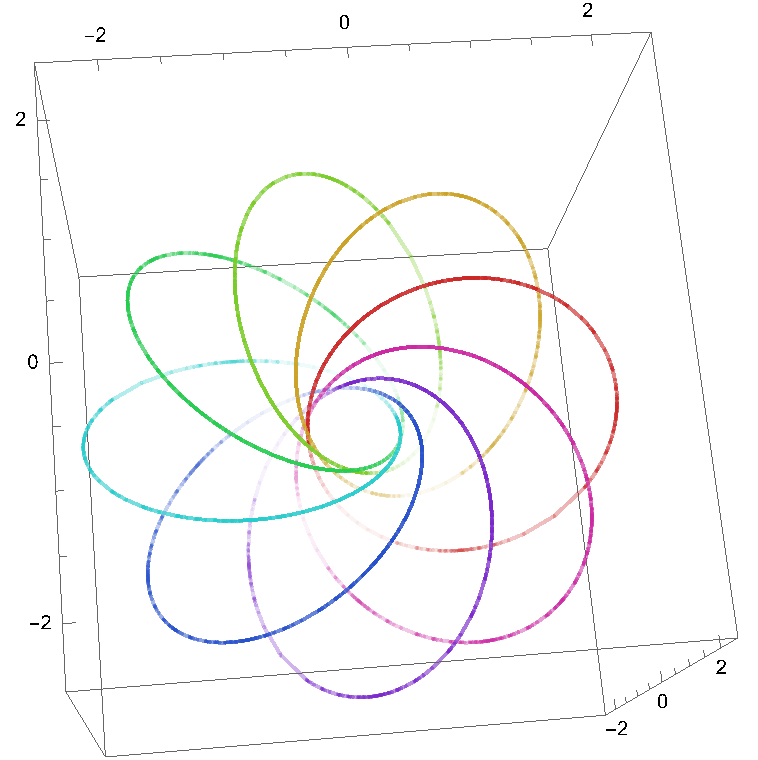
\includegraphics[width=0.5\textwidth]{hopf-fibers.png}
  \caption{Fibers of the Hopf fibration $S^3\to S^2$, drawn after a stereographic projection
  from $(S^3 \setminus \text{north pole}) \to \bR^3$.  
  Here the fibers over $(\cos 2\pi k/8,\sin 2\pi k/8, 0)$ for $k=0,\ldots,7$ are shown. 
}
\end{figure}


\begin{table}[h]
  \[
\begin{array}{c|cccccccccccccccccc}
  k & 0 & 1 & 2 & 3 & 4 & 5 & 6 & 7 & 8 & 9  \\
   \hline
  S^1 & \textcolor{red}{\bZ} & 0 & 0 & 0 & 0 & 0 & 0 & 0 & 0 & 0 \\
  S^2 & \cellcolor{lg} \textcolor{red}{\bZ} & \textcolor{blue}{\bZ} & \bZ_2 & \bZ_2 & \bZ_{12} & \bZ_2 & \bZ_2 & \bZ_3 & \bZ_{15} & \bZ_2  \\
  S^3 & \cellcolor{lg} \textcolor{red}{\bZ} & \cellcolor{lg} \bZ_2 & \bZ_2 & \bZ_{12} & \bZ_2 & \bZ_2 & \bZ_3 & \bZ_{15} & \bZ_2 & (\bZ_2)^2  \\
  S^4 &\cellcolor{lg}  \textcolor{red}{\bZ} & \cellcolor{lg} \bZ_2 & \cellcolor{lg} \bZ_2 & \textcolor{blue}{\bZ} \times \bZ_{12} & (\bZ_2)^2 & (\bZ_2)^2 & \bZ_{24} \times \bZ_3 & \bZ_{15} & \bZ_2  & (\bZ_2)^3\\
  S^5 & \cellcolor{lg} \textcolor{red}{\bZ} & \cellcolor{lg} \bZ_2 & \cellcolor{lg} \bZ_2 & \cellcolor{lg} \bZ_{24} & \bZ_2 & \bZ_2 & \bZ_2 & \bZ_{30} & \bZ_2 & (\bZ_2)^3  \\
  S^6 & \cellcolor{lg} \textcolor{red}{\bZ} & \cellcolor{lg} \bZ_2 & \cellcolor{lg} \bZ_2 & \cellcolor{lg} \bZ_{24} & \cellcolor{lg} 0 & \textcolor{blue}{\bZ} & \bZ_2 & \bZ_{60} & \bZ_{24}\times \bZ_2 & (\bZ_2)^3\\
  S^7 &\cellcolor{lg}  \textcolor{red}{\bZ} & \cellcolor{lg} \bZ_2 & \cellcolor{lg} \bZ_2 & \cellcolor{lg}\bZ_{24} & \cellcolor{lg} 0 &\cellcolor{lg}  0 & \bZ_2 & \bZ_{120} & (\bZ_2)^3 & (\bZ_2)^4 \\
  S^8 & \cellcolor{lg} \textcolor{red}{\bZ} & \cellcolor{lg} \bZ_2 & \cellcolor{lg} \bZ_2 & \cellcolor{lg} \bZ_{24} & \cellcolor{lg} 0 & \cellcolor{lg} 0 & \cellcolor{lg} \bZ_2 & \textcolor{blue}{\bZ}\times \bZ_{120} & (\bZ_2)^4 & (\bZ_2)^5 \\
  S^9 &\cellcolor{lg}  \textcolor{red}{\bZ} & \cellcolor{lg} \bZ_2 & \cellcolor{lg} \bZ_2 & \cellcolor{lg} \bZ_{24} & \cellcolor{lg} 0 & \cellcolor{lg} 0 & \cellcolor{lg} \bZ_2 & \cellcolor{lg} \bZ_{240} & (\bZ_2)^3 & (\bZ_2)^4 \\
  S^{10} &\cellcolor{lg}  \textcolor{red}{\bZ} & \cellcolor{lg} \bZ_2 & \cellcolor{lg} \bZ_2 & \cellcolor{lg} \bZ_{24} & \cellcolor{lg} 0 & \cellcolor{lg} 0 & \cellcolor{lg} \bZ_2 & \cellcolor{lg} \bZ_{240} & \cellcolor{lg} (\bZ_2)^2 & \textcolor{blue}{\bZ}\times (\bZ_2)^3 \\
  S^{11} &\cellcolor{lg}  \textcolor{red}{\bZ} & \cellcolor{lg} \bZ_2 & \cellcolor{lg} \bZ_2 & \cellcolor{lg} \bZ_{24} & \cellcolor{lg} 0 & \cellcolor{lg} 0 & \cellcolor{lg} \bZ_2 & \cellcolor{lg} \bZ_{240} & \cellcolor{lg} (\bZ_2)^2 & \cellcolor{lg} (\bZ_2)^3 \\
  S^{12} &\cellcolor{lg}  \textcolor{red}{\bZ} & \cellcolor{lg} \bZ_2 & \cellcolor{lg} \bZ_2 & \cellcolor{lg} \bZ_{24} & \cellcolor{lg} 0 & \cellcolor{lg} 0 & \cellcolor{lg} \bZ_2 & \cellcolor{lg} \bZ_{240} & \cellcolor{lg} (\bZ_2)^2 & \cellcolor{lg} (\bZ_2)^3 \\
\end{array}
\]
\caption{Table of $\pi_{n+k}(S^n)$ \label{tab:pi_nS^m}}
\end{table}


\begin{table}[ht]
  \[
  \begin{array}{c|cccccccccccccccc}
  G~\setminus~d&2&3&4&5&6&7&8&9&10&11 \\
  \hline
  \hline
  \Sp(1) &\cellcolor{lg}0&\cellcolor{lg} \bZ&\cellcolor{lg} \BZ_2 &\cellcolor{lg}\BZ_2 & \BZ_{12} &\BZ_{2} &\BZ_{2} &\BZ_{3} & \bZ_{15} &\bZ_2\\
  \Sp(2) &\cellcolor{lg}0&\cellcolor{lg}\bZ& \cellcolor{lg} \BZ_2 &\cellcolor{lg}\BZ_2 &\cellcolor{lg} 0 &\cellcolor{lg}\BZ_{} &0 &\cellcolor{lg}0 & \bZ_{120} &\bZ_2\\
  \Sp(3) &\cellcolor{lg}0&\cellcolor{lg} \bZ&\cellcolor{lg} \BZ_2 &\cellcolor{lg}\BZ_2 &\cellcolor{lg} 0 &\cellcolor{lg}\BZ_{} &\cellcolor{lg}0 &\cellcolor{lg}0 &\cellcolor{lg} 0 &\cellcolor{lg} \bZ\\
  \hline
  \SU(3) &\cellcolor{lg}0&\cellcolor{lg} \bZ&\cellcolor{lg}0 &\cellcolor{lg}\BZ &\BZ_{6} &0 &\BZ_{12} &\BZ_{3} & \bZ_{30} & \bZ_4 \\
  \SU(4) &\cellcolor{lg}0&\cellcolor{lg}\bZ&\cellcolor{lg}0 &\cellcolor{lg}\BZ &\cellcolor{lg}0 &\cellcolor{lg}\BZ &\BZ_{24} &\BZ_{2} &   \bZ_{120}\times \bZ_2 & \bZ_4 \\
  \SU(5) &\cellcolor{lg}0&\cellcolor{lg}\bZ&\cellcolor{lg}0 &\cellcolor{lg}\BZ &\cellcolor{lg} 0 &\cellcolor{lg}\BZ &\cellcolor{lg}0 &\cellcolor{lg}\BZ &  \bZ_{120}& 0 \\
  \SU(6) &\cellcolor{lg}0&\cellcolor{lg}\bZ&\cellcolor{lg}0 &\cellcolor{lg}\BZ &\cellcolor{lg} 0 &\cellcolor{lg}\BZ &\cellcolor{lg}0 &\cellcolor{lg}\BZ &  \cellcolor{lg}0 & \cellcolor{lg}\bZ  \\
  \hline
  Spin(7) &\cellcolor{lg}0&\cellcolor{lg}\bZ&\cellcolor{lg}0 &\cellcolor{lg}0 &0 &\BZ_{} &(\BZ_{2})^2 &(\BZ_{2})^2 & \bZ_8 & \bZ\times \bZ_2 \\
  Spin(8) &\cellcolor{lg}0&\cellcolor{lg}\bZ&\cellcolor{lg}0 &\cellcolor{lg}0 &\cellcolor{lg}0 &\BZ_{}^2 &(\BZ_{2})^3 &(\BZ_{2})^3 &\bZ_{24}\times \bZ_8 & \bZ\times \bZ_2    \\
  Spin(9) &\cellcolor{lg}0&\cellcolor{lg}\bZ&\cellcolor{lg}0 &\cellcolor{lg}0 & \cellcolor{lg} 0 &\cellcolor{lg}\BZ_{} &(\BZ_{2})^2 &(\BZ_{2})^2 &   \bZ_8 & \bZ\times \bZ_2\\
  Spin(10) &\cellcolor{lg}0&\cellcolor{lg}\bZ&\cellcolor{lg}0 &\cellcolor{lg}0 & \cellcolor{lg}0 &\cellcolor{lg}\BZ_{} &\cellcolor{lg}\BZ_{2} &\BZ \times \BZ_{2} &  \bZ_4 & \bZ \\
  Spin(11) &\cellcolor{lg}0&\cellcolor{lg}\bZ&\cellcolor{lg}0 &\cellcolor{lg}0 &\cellcolor{lg}0 &\cellcolor{lg}\BZ_{} &\cellcolor{lg}\BZ_{2} &\cellcolor{lg}\BZ_{2} &   \bZ_2 & \bZ\\
  Spin(12) &\cellcolor{lg}0&\cellcolor{lg}\bZ&\cellcolor{lg}0 &\cellcolor{lg}0 &\cellcolor{lg}0 &\cellcolor{lg}\BZ_{} &\cellcolor{lg}\BZ_{2} &\cellcolor{lg}\BZ_{2} &   \cellcolor{lg}0 & \bZ\times \bZ \\
  Spin(13 ) &\cellcolor{lg}0&\cellcolor{lg}\bZ&\cellcolor{lg}0 &\cellcolor{lg}0 &\cellcolor{lg}0 &\cellcolor{lg}\BZ_{} &\cellcolor{lg}\BZ_{2} &\cellcolor{lg}\BZ_{2} & \cellcolor{lg}  0 & \cellcolor{lg}\bZ\\
  \hline
  G_2 &0&\bZ&0 &0 & \BZ_{3} &0 &\BZ_{2} &\BZ_{6} &   0 & \bZ\times \bZ_2\\
  F_4 &0&\bZ&0 &0 &  0 &0 &\BZ_{2} &\BZ_{2} &0 & \bZ\times \bZ_2 \\
  E_6 &0&\bZ&0 &0 &  0 &0 &0 &\BZ & 0&\bZ \\
  E_7 &0&\bZ&0 &0 &  0 &0 &0 &0 &  0 & \bZ\\
  E_8 &0&\bZ&0 &0 &    0 &0 &0 &0 & 0 & 0
  \end{array}
  \]
  \caption{Homotopy groups of simply-connected simple Lie groups $\pi_d(G)$, $2\le d\le 11$.
   \label{tab:pi_nG}}
\end{table}


\end{document}



